\chapter{Przegląd piśmiennictwa}

Choroba Alzheimera nadal nie jest w pełni zrozumiana, jednak dzięki badaniom zdobyto już wiele istotnych informacji na jej temat.
Część z nich opiera się wyłącznie na korelacjach i potwierdzonych powiązaniach z pominięciem przyczyn i konkretnych mechanizmów nimi rządzących, lecz nadal daje nam to wystarczający obraz by przedstawić kompleksowo opis choroby.

\section{Historia, definicja i objawy choroby Alzheimera}

\subsection{Wczesna historia}

Istnienie demencji było znane ludzkości od bardzo dawna.
Pierwsze wzmianki na ten temat pojawiały się już w czasach starożytnej Grecji, a informacje dotyczące jej objawów można odnaleźć nawet wcześniej, w starożytnym Egipcie \cite{boller1998history}.

Natomiast choroba Alzheimera została po raz pierwszy opisana przez niemieckiego lekarza Aloisa Alzheimera, od którego nazwiska została później nazwana.
W roku 1901 neuropatolog zajął się przypadkiem Auguste Deter, pacjentki przyjętej do szpitala psychiatrycznego.
Od jej 51. roku życia zaczęły się stopniowe zmiany osobowości, które następnie przerodziły się w postępujące zaburzenia kognitywne, a ostatecznie w całkowitą apatię \cite{cipriani2011alzheimer}.
W momencie, gdy Alzheimer rozpoczął badania nad nią, pacjentka miała już prawie pięcioletnią historię narastających halucynacji, urojeń, apraksji, zaburzeń pamięci, mowy, społecznych i behawioralnych.

Po śmierci pacjentki lekarz przeprowadził badania mózgu zmarłej, w trakcie których znalazł zmiany i cechy dziś przypisywane omawianej chorobie.
Alzheimer przedstawił swoje kliniczne i patologiczne wyniki na konferencji południowo-zachodnich niemieckich psychiatrów w 1906 roku, następnie opublikował w formie pisemnej w czasopismach medycznych poświęconych psychiatrii \cite{alzheimer1906uber}.

W tym czasie jeszcze sam Alois Alzheimer nie był pewien, czy przypadek Auguste Deter reprezentował nowy zespół chorobowy.
Uważał, że opisał bardzo rzadką przypadłość i najprawdopodobniej wierzył, że była to po prostu szczególna forma demencji starczej \cite{cipriani2011alzheimer}.
Dopiero kilka lat później, po raz pierwszy użyty został termin ``choroba Alzheimera'' (\emph{ang. ``Alzheimer's disease'', często po prostu ``AD''}) w wydanym podręczniku psychiatrii Emila Kraeplina \cite{kraepelin1910psychiatrie}.

Jeszcze w pierwszej połowie XX wieku publikacje podkreślały brak zależności przebiegu choroby Alzheimera od wieku pacjentów.
Pojawiła się również istotna kliniczna debata wokół pytania czy demencja ``przedstarcza'' oraz demencja ``starcza'' (\emph{ang. kolejno ``presenile'' oraz ``senile''}) są tym samym zaburzeniem \cite{jellinger2006alzheimer}.
W połowie wieku pojawiły się pierwsze postulaty mówiące, że (przedstarcze) \emph{AD} oraz demencja starcza są całkowicie odrębnymi jednostkami chorobowymi (choć nowsze badania dojść jednoznacznie pokazują, że tak nie jest).

W latach 60 XX wieku rozpoczęła się nowa era badań bazująca na nowym, bardzo ważnym narzędziu badawczym -- mikroskopii elektronowej.
Dzięki niej możliwe było zbadanie struktury komórek nerwowych i ich połączeń, a także zbadanie struktury i składu splotów nerwowych znajdujących się w mózgu.
Takich opisów jako jeden z pierwszych dostarczył w 1963 roku Kidd, który opisał zmiany w strukturze splątków neurofibrylarnych oraz blaszek amyloidowych \cite{kidd1963paired}.

Od tego czasu choroba progresywnie zyskiwała coraz większą uwagę ze strony środowiska naukowego, a także społeczeństwa.
W 1974 roku rząd Stanów Zjednoczonych Ameryki powołał do istnienia Narodowy Instytut ds. Starzenia się (\emph{ang. National Institute on Aging, NIA}), który od tego czasu finansuje badania nad chorobą Alzheimera \cite{marx1974aging}.
W 1980 roku powstało ``Stowarzyszenie Choroby Alzheimera i Pokrewnych Zaburzeń'' (\emph{ang. Alzheimer's Disease and Related Disorders Association, ADRDA}), organizacja non-profit, która dziś znana jest jako ``Stowarzyszenie Choroby Alzheimera'' (\emph{ang. Alzheimer's Association, AA}).
Wraz z rosnącą świadomością społeczną wzrastało także finansowanie, dzięki czemu choroba jeszcze 30 lat temu uznawana za całkiem nieuleczalną i nie do powstrzymania czy spowolnienia, dziś jest jedną z najbardziej intensywnie badanych chorób neurodegeneracyjnych z prospektami na walkę z nią w niedalekiej przyszłości.

Mimo tych wielu obecnych badań, nadal pozostaje wiele czynników wciąż niepoznanych i nie ma jednoznacznej odpowiedzi na pytanie co jest przyczyną choroby Alzheimera.
Wciąż brakuje również skutecznych metod leczenia, które mogłyby zatrzymać jej postęp lub spowolnić go w znaczący sposób.

\subsection{Współczesna definicja choroby Alzheimera}

W celu lepszego zrozumienia choroby Alzheimera, warto najpierw przyjrzeć się dwóm definicjom -- czym jest demencja oraz czym jest choroba Alzheimera -- jako, że terminy te często w świadomości publicznej są utożsamiane, co nie jest prawdą, choć pojawiają się między nimi istotne powiązania.

Demencja (inaczej \emph{otępienie}) to znacznie ogólniejszy termin określający utratę pamięci, zdolności językowych, umiejętności rozwiązywania problemów i utrudnienie innych czynności poznawczych, które są na tyle poważne, że przeszkadzają w codziennym życiu.
Nie odnosi się w żadnym wypadku do naturalnego procesu starzenia się i nie należy drobnych problemów z pamięcią czy zapominalstwa z nią mylić.
Demencja jest też objawem, a nie chorobą i może być spowodowana przez wiele różnych chorób i zaburzeń.

Choroba Alzheimera jest jedną z wielu chorób, które mogą prowadzić do demencji.
Odpowiada ona za między 60\% a 80\% przypadków demencji, co czyni ją najczęstszą przyczyną otępienia \cite{what-is-alzheimers:2023}.
Obecnie klinicyści używają terminu \emph{AD} -- choroba Alzheimera -- w odniesieniu do zespołu chorobowego, który objawia się charakterystycznym postępującym zaburzeniem amnezyjnym z późniejszym pojawianiem się innych zmian poznawczych, behawioralnych i neuropsychiatrycznych, które upośledzają funkcje społeczne i czynności życia codziennego \cite{cummings2004alzheimer}.

Mimo, że choroba Alzheimera jest najczęstszą przyczyną demencji, to jednak nie jest z nią tożsama.
Drugą najczęstszą przyczyną jest demencja naczyniowa, która jest spowodowana uszkodzeniem naczyń krwionośnych w mózgu, najczęściej w wyniku udaru mózgu.


\subsection{Objawy choroby Alzheimera i stadium demencji}

Objawy choroby Alzheimera są bardzo zróżnicowane i zależą od stadium choroby.
Dodatkowo wczesne objawy często są mylone z naturalnym procesem starzenia się, co utrudnia wczesną diagnozę.

Ogólnie rzecz biorąc, objawy choroby Alzheimera można podzielić na 3 główne etapy powiązane ze stadium choroby \cite{alzheimers-symptoms:2021}:

\begin{itemize}

  \item Wczesne objawy

        W początkach rozwijającej się choroby głównym symptomem są zaniki pamięci.
        Można tutaj wymienić między innymi zapominanie o niedawnych rozmowach lub wydarzeniach, gubienie przedmiotów, zapominać nazw miejsc i rzeczy, powtarzanie się, trudności w znalezieniu właściwego słowa czy podejmowaniu decyzji.
        Łatwo zauważyć, że są to objawy, które mogą pojawić się w mniejszym stopniu u każdego człowieka, w tym w pełni zdrowego, co znacznie utrudnia wczesną diagnozę -- nasilenia się tych objawów są często mylone z naturalnym procesem starzenia się.

  \item Objawy w średnim stadium

        Narastają przypadku dezorientacji - na przykład gubienie się, błądzenie czy brak świadomości pory dnia.
        Chory może powtarzać czynności, mieć urojenia, odczuwać paranoję, zaburzony jest sen.
        AD może również wpływać na psychikę, powodując częste zachwiania nastroju, niepokój, frustrację czy depresję \cite{li2014behavioral}.
        Niebezpieczne mogą być także problemy z percepcją -- ocena odległości czy uświadamiane widzenie lub słyszenie.

        Wraz z rozwojem choroby Alzheimera, problemy z pamięcią będą się pogarszać.
        Pogłębiają się problemy z zapamiętywaniem imion, nawet tych osób, które zna się od dawna.
        Mogą pojawiać się także trudności w rozpoznawaniu miejsc i osób.
        Ciężkim, możliwym objawem pojawiającym się w średnim stadium jest także afazja, czyli zaburzenia mowy i języka.

        Na tym etapie osoba cierpiąca na chorobę Alzheimera zazwyczaj potrzebuje wsparcia w codziennym życiu.

  \item Późniejsze objawy

        W późniejszych stadiach choroby Alzheimera objawy stają się coraz bardziej nasilone i mogą być w znacznym stopniu wpływać na osobę chorą, a także jej opiekunów, przyjaciół i rodziny.

        Mogą pojawiać się halucynacje i urojenia, zanikające lub nasilające się wraz z postępem choroby.
        Czasami osoby cierpiące na chorobę Alzheimera mogą być agresywne, wymagające i podejrzliwe w stosunku do otoczenia.

        W miarę postępu choroby Alzheimera może również rozwinąć się szereg innych objawów, takich jak dysfagia (trudności z połykaniem), nietrzymanie moczu czy stolca, problemy z poruszaniem się bez pomocy, fizyczna utrata masy ciała, a także stopniowa i często szybka utrata zdolności poznawczych -- w tym mowy \cite{joe2019cognitive}.
        Znacznie pogłębiają się problemy z krótko- i długoterminową.

        W ciężkich stadiach choroby Alzheimera ludzie mogą potrzebować całodobowej opieki oraz pomocy w jedzeniu, poruszaniu się i pielęgnacji osobistej.

\end{itemize}

\section{Diagnoza choroby Alzheimera}

Mimo, że choroba Alzheimera nadal nie jest w pełni zrozumiana i zbadana oraz wciąż nie ma skutecznych metod jej leczenia, to obszar diagnozy i wczesnego wykrywania choroby jest bardzo dobrze rozwinięty.
Powstało wiele metod i narzędzi diagnostycznych, które pozwalają na wczesne wykrycie choroby.

\subsection{Metody kliniczne diagnostyki choroby Alzheimera}

Między rokiem 1960 a 1985 wprowadzono kilka różnych kategorii obiektywnych klinicznie narzędzi diagnostyki choroby Alzheimera, wiele z nich potwierdzonych w autopsji \cite{khachaturian2006diagnosis}.
Były to między innymi:

\begin{itemize}

  \item \emph{Mini-Mental State Examination} (w skrócie \emph{MMSE}, potocznie mini-mental) -- jest to zaprojektowany w 1975 roku test oceny demencji oraz jej stopnia w formie szybkiego badania, najczęściej krótszego niż 5 minut.
        Mini-mental jest narzędziem przesiewowym (ang. \emph{screening}), to jest -- nie jest dokładne i jednoznaczne, ale jego negatywny wynik daje podstawy przypuszczać prawdopodobną utratę zdolności kognitywnych i wszcząć
        głębsze, kliniczne badania w celu potwierdzenia wstępnej diagnozy.

        W wyniku tego badania uzyskuje się między 0 a 30 punktów, gdzie wraz z malejącą zdobytą ilością rośnie domniemany stopień demencji.
        27 punktów oraz powyżej oznacza wynik prawidłowy, 24 i w górę to niedemencyjne zaburzenia poznawcze, 19 wzwyż sugerują demencję łagodną, od 11 do 18 demencję średniego stopnia, a poniżej 10 demencję głęboką.

        Niedawne badania nad skutecznością MMSE na przestrzeni różnych kategorii stwierdzały jej czułość (sensitivity) między 23\% a 76\%, a jej specyficzność (specificity) między 40\% a 90\% \cite{arevalo2015mini}.
        Nie jest to więc wynik wysoki, jednakże wciąż jest to istotne narzędzie używane w praktyce klinicznej, głównie ze względu na jego prostotę i szybkość.

  \item \emph{Short Blessed Test} (w skrócie \emph{SBT}) -- badanie opublikowane do użytku w 1983 roku skupiające się na orientacji, pamięci i koncentracji \cite{katzman1983validation}.
        Według samych autorów przeznaczone do wykrywania wczesnych zaburzeń poznawczych, nie samej diagnozy choroby Alzheimera.
        Wszelkie wyniki sugerujące demencję wymagają dalszych badań.

  \item \emph{Clinician's Interview-Based Impression of Change plus caregiver input} (w skrócie \emph{CIBIC+}) -- zaproponowane i wymagane przez amerykańską Agencję Leków i Żywności (ang. \emph{FDA}, \emph{Food and Drug Administration}) podejście do przeprowadzania badań nad lekami na chorobę Alzheimera i demencję, który ma pozwalać na uzyskiwanie mierzalnych klinicznie danych potrzebnych do oceny skuteczności badanych środków \cite{joffres2000qualitative}.
        Najczęściej praktykowanym testem implementującym założenia CIBIC+ jest \emph{Alzheimer's Disease Cooperative Study -- Clinical Global Impression of Change} (w skrócie \emph{ADCS-CGIC}) z roku 1990.

  \item \emph{Clinical Dementia Rating} (w skrócie \emph{CDR}) -- skala numeryczna używana do ilościowego określenia nasilenia się objawów demencyjnych i skategoryzowania choroby w określonym "stadium".
        Wynik w tej skali otrzymuje się jako rezultat przeprowadzenia wywiadu z pacjentem opracowanego w 1993 roku przez Morrisa i jego współpracowników, lekarzy z Washington University School of Medicine \cite{morris1993clinical}.

        CDR uważany jest za test zdolny do rozpoznania bardzo łagodnych upośledzeń, co przeważnie nie było możliwe w poprzednich testach klinicznych dotyczących choroby Alzheimera.
        Ma on jednak słabe strony, w tym najważniejszy -- długi czas potrzebny na przeprowadzenie całościowego wywiadu i co za tym idzie jest względnie niezdolny do uchwycenia zmian w czasie.
        Dodatkowo polega on na subiektywnej ocenie lekarza, co może prowadzić do błędów.

  \item \emph{Alzheimer's Disease Assessment Scale -- Cognitive Subscale} (w skrócie \emph{ADAS--Cog}) -- test kliniczny, który mierzy zmiany w funkcjonowaniu poznawczym pacjenta i nasilenie objawów demencji.
        Jest połową większego testu, \emph{Alzheimer's Disease Assessment Scale} (w skrócie \emph{ADAS}), który składa się z dwóch części: \emph{ADAS--Cog} oraz \emph{ADAS--Noncog}.
        ADAS--Cog zawiera 11 pytań, które oceniają pamięć, orientację, rozumienie, umiejętności wykonawcze i język.
        Do dnia dzisiejszego jest on na szeroką skalę używany w badaniach klinicznych nad lekami na demencję czy chorobę Alzheimera i uważany za najlepszy standard  ocenie leczenia przeciw otępieniu \cite{connor2008administration}.

\end{itemize}

Większość tego typu badań ma charakter niekonkluzywny i nie są w stanie jednoznacznie potwierdzić czy wykluczyć chorobę Alzheimera.
Wymagają one dalszych badań, które mogą być zarówno kliniczne, jak i laboratoryjne.
Część z nich jednak -- w szczególności ostatni z wymienionych, \emph{ADAS--Cog} -- są na tyle dokładne, że do dziś są bardzo szeroko używane w badaniach klinicznych nad chorobą Alzheimera.
A z kolei wszystkie są wystarczająco skuteczne, by być podstawą do podjęcia decyzji i przeprowadzeniu znacznie dokładniejszych badań laboratoryjnych.
Takimi dokładnymi badaniami biologicznymi mogą być pośmiertne badania neuropatologiczne, ale także możliwe jest w trakcie życia pacjenta badanie biomarkerów wskazujących na chorobę Alzheimera \cite{mantzavinos2017biomarkers}.

Nowoczesne uniwersalne narzędzia diagnostyczne są również bardzo przydatne w badaniach nad chorobą Alzheimera, w szczególności możliwość dokładnego obrazowania mózgu.

\subsection{Metody obrazowania mózgu w diagnostyce choroby Alzheimera}

Sugestie dotyczące przydatności i skuteczności nowych technik obrazowania mózgu w diagnostyce choroby Alzheimera pojawiły się już w latach 80 XX wieku \cite{mcgeer1986brain}.
Testowano wykorzystanie tomografii komputerowej (\emph{CT}), rezonansu magnetycznego (\emph{MRI}), pozytonowej tomografii emisyjnej (\emph{PET}) oraz pojedynczej emisji fotonów (\emph{SP}).
Autorzy wskazywali jednak, że skany tomografii komputerowej i rezonansu magnetycznego ujawniają uogólniony proces zanikowy kory mózgowej, który nasila się wraz z wiekiem i mimo, że proces zanikowy jest bardziej nasilony w chorobie Alzheimera, to jednak nie może być stosowany jako metoda diagnostyczna, ponieważ nie występuje w każdym przypadku.
Dodali też, że zmian nie można przewidzieć z użyciem tych dwóch wspomnianych metod.

Nowsze prace jednak nie są tak rygorystyczne w stosunku do metod obrazowania mózgu i zaznaczają, że zarówno pierwotnie używana tomografia komputerowa, a także następnie wprowadzony rezonans magnetyczny były i są z powodzeniem używane w diagnostyce choroby Alzheimera \cite{johnson2012brain}.
Co więcej, funkcjonalny rezonans magnetyczny (\emph{fMRI}) czy pozytonowa tomografia emisyjna (\emph{PET}) potrafiły wykazać charakterystyczne zmiany w mózgach pacjentów z \emph{AD} w stadiach nawet przedobjawowych,
Żadna z metod obrazowania nie może służyć wszystkim celom, ponieważ każda z nich ma unikalne mocne i słabe strony.

\begin{figure}[ht]
  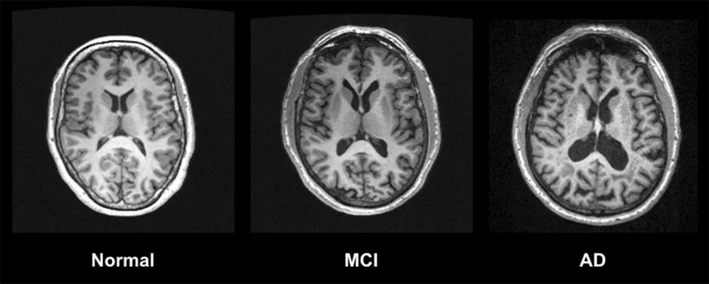
\includegraphics[width=\textwidth]{mri-images-of-normal-mci-and-ad-brains}
  \caption[Obrazy porównawcze rezonansu magnetycznego mózgów pacjentów z chorobą Alzheimera oraz zdrowych]{Obrazy porównawcze rezonansu magnetycznego mózgów pacjentów zdrowych, z łagodnym zaburzeniem poznawczym (ang. \emph{Mild Cognitive Impairment}, lub \emph{MCI}) oraz z chorobą Alzheimera \emph{AD}. Grafika pochodząca z artykułu dla ADNI (\emph{Alzheimer's Disease Neuroimaging Initiative}) \cite{chandra2019magnetic}.}
  \label{mri-images-of-normal-mci-and-ad-brains}
\end{figure}

Przykładowe obrazowanie mózgów przy użyciu rezonansu magnetycznego przedstawia \hyperref[mri-images-of-normal-mci-and-ad-brains]{rysunek \ref*{mri-images-of-normal-mci-and-ad-brains}}, gdzie przedstawione są kolejno od lewej: obraz mózgu osoby zdrowej obraz osoby z lżejszą jednostką chorobową łagodnego zaburzenia poznawczego (ang. \emph{Mild Cognitive Impairment}, lub \emph{MCI}) oraz obraz mózgu osoby z chorobą Alzheimera \emph{AD}.
Jak widać, mózg osoby z chorobą Alzheimera jest znacznie bardziej zdegenerowany, a także posiada charakterystyczne zmiany w kształcie i strukturze.

Bardzo świeże prace z 2022 roku opisują, że obecnie neuroobrazowanie znajduje się w ścisłej czołówce metod pomocnych w diagnozowaniu choroby Alzheimera (\emph{AD}), a także innych wszelkich innych rodzajów demencji, takich jak otępienie czołowo-skroniowe, otępienie naczyniowe i otępienie z ciałami Lewy'ego (\emph{DLB}) \cite{scheltens2022imaging}.
Niedawno sformułowane przez Dubois i współpracowników kryteria badawcze dla wczesnej choroby Alzheimera wyraźnie wymieniają obrazowanie rezonansu magnetycznego (\emph{MRI}) i pozytonową tomografię emisyjną (\emph{PET}) dla \emph{AD} i są przykładem rozwoju nowego procesu diagnostycznego.
Autorzy sugerują, że wkrótce neuroobrazowanie zostanie włączone do kryteriów diagnostycznych dla różnych rodzajów demencji.

\subsection{Nowoczesne metody detekcji choroby Alzheimera z użyciem uczenia maszynowego}
\label{modern-detection-methods-for-alzheimers-using-machine-learning}

Diagnostyka choroby Alzheimera miała duże skoki rozwojowe wraz z powstawaniem nowych technologii i metod badawczych.
Już w połowie lat 90 XX wieku pojawiły się pierwsze prace naukowe próbujące wykorzystać rozwijającą się dziedzinę uczenia maszynowego przy detekcji demencji.
Te pierwsze próby opierały się jednak nie na obrazach, ale na analizie danych klinicznych i rezultatów testów psychometrycznych \cite{datta1996applying}.
Rezultaty pokazały, że już te proste podejścia mają skuteczność nieco lepszą niż kwestionariusze zaprojektowane do ręcznej analizy zebranych danych.

Rosnąca popularność neuroobrazowania w diagnostyce choroby Alzheimera oraz dalszy rozwój technik uczenia maszynowego i sztucznej inteligencji doprowadziły do powstania wielu prac naukowych, które łączą te dwa obszary.

W 2007 roku podjęto próbę analizy kształtu hipokampu u pacjentów z chorobą Alzheimera z użyciem technik uczenia maszynowego \cite{li2007hippocampal}.
W wyniku uznano, że subtelne i przestrzennie złożone wzorce deformacji hipokampa pomiędzy pacjentami posiadającymi AD a zdrowymi osobami kontrolnymi można wykryć za pomocą metod uczenia maszynowego.

Dalsze badania sprawdzały skuteczność technik klasyfikacji w uczeniu maszynowym obrazów rezonansu magnetycznego w celu detekcji choroby Alzheimera \cite{herrera2013classification}.
Klasyfikacja miała być binarna, czyli obrazy były przydzielane do kategorii osób zdrowych lub kategorii osób z chorobą Alzheimera, bez podziału na stadium choroby.
Powstały model miał służyć jako pomoc we wczesnym sygnalizowaniu potencjalnych wskaźników choroby Alzheimera.

Nowe prace analizowały wykorzystywane do celów diagnostyki metody uczenia maszynowego na przestrzeni lat 2005 do 2019 \cite{tanveer2020machine}.
Zamknięto pojawiające się techniki w 3 kategoriach: maszyny wektorów nośnych (ang. \emph{Support Vector Machine}, \emph{SVM}), sztuczne sieci neuronowe (ang. \emph{Artificial Neural Network}, \emph{ANN}) oraz uczenie głębokie (ang. \emph{Deep Learning}, \emph{DL}).
Jak się okazuje, najwięcej prac naukowych używało technik maszyn wektorów nośnych \emph{SVM} ze względu na ich powtarzalność i solidność wyników, nie cierpią one bowiem na problemy związane z lokalnymi minimami.
Jednak sieci neuronowe są bardziej wszechstronne, jeśli chodzi o przyrostowe uczenie się i modelowanie danych sekwencyjnych.
Najbardziej obiecująca jednak była technika uczenia głębokiego, dzięki której można modelować bardzo złożone dane z dużą dokładnością.

W tę właśnie stronę poszli autorzy późniejszej pracy, którzy używając obrazów rezonansu magnetycznego MRI wyszkolili głęboki model dla detekcji choroby Alzheimera \cite{ebrahimi2021deep}.
Wykorzystali oni konwolucyjne głębokie sieci neuronowe i różne rodzaje sieci rekurencyjnych bazowanych na wstępnie wytrenowanym modelu ResNet-18.
Otrzymali bardzo obiecujące wyniki i model, który osiągnął maksymalną wydajność klasyfikacji z dokładnością, czułością i swoistością na poziomie około 92\%.

Innym bardzo ciekawym podejściem do detekcji choroby Alzheimera przy użyciu uczenia maszynowego była próba wykorzystania cech spektrogramu wyodrębnionych z danych mowy pacjentów zamiast trudnych do zdobycia obrazów medycznych \cite{liu2020new}.
Autorom tej pracy udało się osiągnąć dokładność poziomu $86.1\%$ w klasyfikacji osób zdrowych i z chorobą Alzheimera, co jest dodatkowo obiecujące biorąc pod uwagę dostępność wykorzystanych danych.

\section{Uczenie maszynowe i techniki klasyfikacji}

W celu lepszego zrozumienia, dlaczego i w jaki sposób uczenie maszynowe może być bardzo przydatnym narzędziem w diagnostyce choroby Alzheimera, a także całym ogólniej w obszarze medycyny i diagnostyki, warto przyjrzeć się na czym polega i jakie są jego podstawowe techniki.

\subsection{Generalna definicja uczenia maszynowego}

Uczenie maszynowe (często w skrócie \emph{ML}, z ang. \emph{Machine Learning}) jest pojęciem bardzo szerokim i z natury interdyscyplinarnym, natomiast w najpopularniejszym użyciu odnosi się do kategorii sztucznej inteligencji, która pozwala komputerom ``myśleć'' i uczyć się we własnym zakresie.
Sam termin został po raz pierwszy użyty przez Arthura Samuela w 1959 roku, który to zdefiniował uczenie maszynowe jako dziedzinę studiów, która daje komputerom możliwość uczenia się bez ich bezpośredniego programowania \cite{samuel1959some}.

Taka definicja uczenia maszynowego, mimo, że ogranicza się do jednej z wielu dziedzin potencjalnie zaliczanych do tej kategorii, jest bardzo ogólna i nie precyzuje dokładnie co to znaczy ``uczyć się'' ani jak takie uczenie się miałoby być manifestowane.
Jest to zabieg celowy, ponieważ -- w przeciwieństwie do tego, co pozwalałyby sądzić najpopularniejsze obecnie metody uczenia maszynowego -- nie jest to jedynie zbiór badań nad sieciami neuronowymi i systemami ekspertowymi.
Wspomniana definicja jednak jest zbyt ogólna, by móc powiedzieć o niej coś więcej bez bazowania na przykładowych technikach i algorytmach.

Aby sformalizować pewne uniwersalne właściwości technik uczenia maszynowego, zaproponowany został podstawowy model uczenia maszynowego.
W nim uczenie maszynowe zostało zaprezentowane jako proces składający się z czterech głównych elementów: środowiska, uczenia, repozytorium oraz wykonania \cite{wang2009brief}.
Wygląd takiego modelu został przedstawiony na \hyperref[fig:basic-model-of-machine-learning]{rysunku \ref*{fig:basic-model-of-machine-learning}}.

\begin{figure}[ht]
  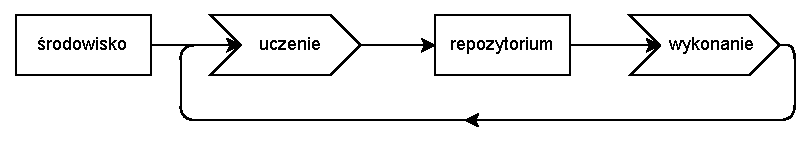
\includegraphics[width=\textwidth]{basic-model-of-machine-learning}
  \caption[Podstawowy model uczenia maszynowego]{Podstawowy model uczenia maszynowego zaadoptowany z pracy Hua Wang, Cuiqin Ma oraz Lijuan Zhou \cite{wang2009brief}. Bloki prostokątne oznaczają systemy a bloki procesowe (przypominające strzałki) oznaczają procesy.}
  \label{fig:basic-model-of-machine-learning}
\end{figure}

\begin{itemize}

  \item W modelu tym ``środowisko'' jest zewnętrznym zbiorem danych, które dostarczane są w pewnej bliżej nieokreślonej formie, reprezentuje źródła informacji zewnętrznych.
        Może to być na przykład zbiór obrazków przedstawiających odręcznie zapisane cyfry arabskie ręcznie oznaczonych rzeczywistą odpowiadającą im cyfrą przez człowieka.
        Mogą to być jednak także wszelkie inne dane pochodzenia zewnętrznego względem systemu uczenia maszynowego a które służą za podstawę do dalszego jego działania i kluczowego procesu uczenia się.


  \item Drugim czynnikiem tego modelu jest ``uczenie'', które jest procesem przetwarzającym informacje zewnętrzne na wiedzę.
        Terminy tutaj występujące są abstrakcją i mogą oznaczać wiele różnych rzeczy, w zależności od konkretnej omawianej techniki.
        Przykładowo w sztucznych sieciach neuronowych uczenie jest realizowane przez algorytm propagacji wstecznej błędu.
        Niezależnie od implementacji, wiedza jako szeroko pojęty rezultat uczenia jest trafia następnie do przechowania w repozytorium.

  \item Trzeci blok modelu, ``repozytorium'', jest miejscem przechowywania ogólnych zasad, które następnie kierują częścią działań wykonawczych systemu uczenia maszynowego.
        W przypadku sztucznych sieci neuronowych takim repozytorium jest sama struktura sieci oraz wagi połączeń między neuronami.
        Jest to szczególnie ciekawy przypadek, gdzie wiedza ta jest przechowywana w formie w zasadzie niedostępnej i niezrozumiałej dla człowieka, gdzie jej wydobycie jest bardzo trudnym zadaniem \cite{boger1997knowledge}.

  \item Ostatni blok modelu to ``wykonanie'', czyli proces, w którym system uczenia maszynowego wykorzystuje zgromadzoną w repozytorium wiedzę do podejmowania decyzji w kontekście problemu, który ma rozwiązać.
        Wynik działania procesu wykonawczego trafia później z powrotem do procesu uczenia, gdzie razem z dalszymi danymi pochodzącymi ze ``środowiska'' jest wykorzystywany do dalszego rozwoju wiedzy.

\end{itemize}

Cały proces zapętla się i pozwala na inkrementacyjne poprawianie wiedzy systemu uczenia maszynowego, aż do osiągnięcia pożądanej skuteczności procesu wykonawczego.
Tak przedstawiony model jest dużą abstrakcją pozostawiającą szczegóły implementacyjne i działania poszczególnych bloków poszczególnym technikom uczenia maszynowego, ale pozwala wyciąganie wniosków całościowych na temat uczenia maszynowego w pracach natury teoretycznej.

Jednak dążąc do lepszego poznania uczenia maszynowego od strony praktycznej, najlepiej jest przyjrzeć się kategoriom technik uczenia maszynowego, które są najczęściej wykorzystywane.

\subsection{Kategorie technik uczenia maszynowego}

Tradycyjnie wyróżnić można trzy paradygmaty ``uczenia'', na które dzieli się szerzej pojęte uczenie maszynowe.
Podział ten bazuje bezpośrednio na rozróżnieniu rodzajów sygnału -- danych dostarczanych do systemu uczenia maszynowego -- oraz informacji zwrotnej przekazywanej systemowi.
Te aspekty z kolei pośrednio wpływają na to, w jaki sposób w ogóle tego typu algorytm się zachowuje i jakie są jego możliwości oraz predyspozycje.
Kategorie te to:

\begin{itemize}

  \item \emph{Uczenie nadzorowane} (ang. \emph{supervised learning}) --
        algorytmy tego typu opierają się na analizie (czy przyswajaniu) zbiorów danych składających się zarówno z sygnału wejściowego, jak i opisanej już informacji zwrotnej.
        Dane wejściowe mogą być w dowolnej postaci, tekstowej, liczbowej, obrazkowej, dźwiękowej -- cokolwiek co może zostać zakodowane w sposób, w jaki algorytm reprezentuje dane.

        Co wyróżnia tę kategorię wśród pozostałych to fakt, że częścią danych przekazywanych do algorytmu jest także informacja na temat oczekiwanego wyjścia, zachowania się modelu.
        Przekazujemy algorytmowi to, jak powinien na podane dane wejściowe zareagować, a proces jego uczenia polega na dopasowaniu się do tych oczekiwań.

        Uczenie nadzorowane jest czasem nazywane także \emph{klasyfikacją} lub \emph{uczeniem indukcyjnym}, chociaż nie są to terminy ściśle równoważne.
        Pojawiają się jednak, ponieważ algorytmy tego typu przypominają rozumowanie indukcyjne, które polega na wyciąganiu ogólnych wniosków na podstawie konkretnych przykładów.
        Dodatkowo są szczególnie przydatne w zadaniach klasyfikacyjnych, w których radzą sobie bardzo dobrze \cite{hastie2009overview}.

        Do zadań klasyfikacyjnych wymagana jest możliwość podzielenia zbioru danych wejściowych na kategorie, gdzie każdy element przynależy do jednej z nich.
        Jednak uczenie nadzorowane także dobrze radzi sobie z problemami regresji, czyli przewidywania wartości liczbowych na podstawie danych wejściowych.
        Wtedy wyjściem nie jest dyskretna kategoria, ale liczba rzeczywista, gdzie dozwolony jest pewien margines błędu -- algorytm ma dążyć jak najbliższej prawdziwej oczekiwanej wartości, jednak nie musi jej dokładnie osiągnąć.
        Przykładem może być system przewidywania cen nieruchomości na podstawie różnych cech mogących na nią wpływać.

        Systemu uczenia nadzorowanego nie potrafią jednak funkcjonować w izolacji -- potrzebują \emph{nadzoru}, zewnętrznej pomocy w postaci poprawnie opisanych lub skategoryzowanych danych wejściowych.
        W praktyce oznacza to, że uczenie nadzorowane jest zależne od człowieka, który musi dostarczyć algorytmowi dane wejściowe wraz z opisami, które często z angielskiego nazywane są \emph{labels}.
        Mimo skuteczności są więc ograniczane przez ilość danych, jaką jesteśmy w stanie dostarczyć, a także przez to, jak dobrze są one opisane.

        Popularnymi przykładami algorytmów uczenia nadzorowanego są między innymi \emph{regresja logistyczna} oraz \emph{k-najbliższych sąsiadów}.


  \item \emph{Uczenie nienadzorowane} (ang. \emph{unsupervised learning}) --
        systemy uczenia maszynowego tego typu różnią się od uczenia nadzorowanego w głównej mierze brakiem informacji zwrotnej.

        Otrzymują również zbiór danych wejściowych w dowolnej postaci, jednak nie są one opisane, nie wiemy odgórnie jak powinien zachować się algorytm na ich podstawie.

        Celem działania algorytmów uczenia nienadzorowanego jest znalezienie w nieopisanych danych wejściowych struktury i prawidłowości, na przykład ich zgrupowanie lub klasteryzacja (ang. \emph{clustering}) -- bezpośrednie wywnioskowanie bliżej nieokreślonych cech danych bez wsparcia z zewnątrz \cite{hastie2009unsupervised}.

        W uczeniu maszynowym tego typu w przeciwieństwie do uczenia nadzorowanego system zamiast reagować na informacje zwrotne powstałe poprzez porównanie opisu danych z wyjściem, algorytmy uczenia nienadzorowanego identyfikują podobieństwa w danych i reagują na podstawie obecności lub braku takich podobieństw w każdym nowym fragmencie zbioru wejściowego.

        Algorytmy uczenia nienadzorowanego są często wykorzystywane do analizy danych, w szczególności do wykrywania anomalii, czyli elementów zbioru danych, które wyróżniają się na tle pozostałych.

        Przykładem algorytmu uczenia nienadzorowanego jest algorytm centroidów, nazywany też algorytmem \emph{k-średnich} (ang. \emph{k-means}), który mimo swoich wad jest jednym z najpopularniejszych algorytmów klasteryzacji \cite{ahmed2020k}.
        Przez swoją nazwę jest często mylony lub błędnie utożsamiany z nadzorowanym podejściem k-najbliższych sąsiadów, jednak jest to zupełnie inny, niepowiązany algorytm.

  \item \emph{Uczenie przez wzmacnianie} (ang. \emph{reinforcement learning}) --
        podejście tego typu nieco różnią się od dwóch poprzednich, ponieważ nie są one zależne od predefiniowanego zbioru danych wejściowych, a od \emph{środowiska}, w którym algorytm się znajduje.
        Opierają się na ``nagradzaniu'' systemu za zachowania, które są pożądane i/lub ``karaniu'' za te niepożądane.

        Tym samym systemy takie są bliżej działania bazującego na modelu opartym na agentach (ang. \emph{agent-based model}, \emph{ABM}).
        Jest to model obliczeniowy służący do symulacji działań i interakcji autonomicznych agentów w celu zrozumienia zachowania systemu i tego, co rządzi jego wynikami.
        W omawianym kontekście oznacza to, że uczony przez wzmacnianie system jest traktowany jako ``agent'' w szeroko rozumianym środowisku, z którym wchodzi w różnego rodzaju interakcje.

        Ogólne założenia uczenia przez wzmacnianie przypominają nieco proces uczenia się, który widzimy u zwierząt i ludzi.
        Agent (system) jest umieszczany w środowisku, w którym może wykonywać pewne akcje.
        Wykonywane przez niego akcje prowadzą do pewnych rezultatów odbieranych przez niego jako nagrody lub kary.
        Otrzymywanie pozytywnych informacji zwrotnych -- nagród -- zachęca agenta do powtarzania akcji, które doprowadziły do ich otrzymania, a otrzymywanie negatywnych informacji zwrotnych -- kar -- zachęca do unikania prowadzących do nich czynności

        Agent skonstruowany jest tak, by chcieć maksymalizować otrzymywane nagrody, a minimalizować kary.
        Nazywane to jest funkcją nagrody (ang. \emph{reward function}).
        Dąży do tego sposobem, który w uproszczeniu można nazwać metodami prób i błędów.

        Przykładem algorytmów uczenia przez wzmacnianie jest metoda Monte Carlo.
        Jest to metoda statystyczna, która wykorzystuje powtarzalne losowania do rozwiązywania problemów, których rozwiązanie jest trudne lub niemożliwe do znalezienia w inny sposób.
        Agent ``próbkuje'' wykonywanie pewnej akcji i uśrednia uzyskane rezultaty -- wartości nagród/kar.
        Następnie uśredniony rezultat osiągnięty w trakcie trwania całości ``epizodu'', czyli pewnego konkretnego zdarzenia, jest wykorzystywany do zmiany zachowania agenta w przyszłości \cite{thrun2000reinforcement}.

\end{itemize}

W kontekście detekcji różnych jednostek chorobowych w medycynie, w tym choroby Alzheimera, najczęściej wykorzystywane są techniki uczenia nadzorowanego.
Pomimo, że uczenie nienadzorowane również dobrze sprawdza się w niektórych przypadkach \cite{raza2021tour} oraz uczenie przez wzmacniane także znajduje swoje zastosowania \cite{zhou2021deep}, to uczenie nadzorowane nadal sprawuje się najlepiej ze względu na naturę danych i problemów jakie najczęściej się w tym obszarze pojawiają.

Warto także dodać, że najnowsze popularne i bardzo obiecujące podejście -- tak zwane \emph{samo-nadzorowane uczenie maszynowe} (ang. \emph{self-supervised machine learning}) -- jest w istocie połączeniem technik uczenia nadzorowanego i nienadzorowanego i jest w stanie wykorzystać zalety obu tych podejść \cite{krishnan2022self}.

\subsection{Podstawowe algorytmy klasyfikacji}

Algorytmów wykorzystywanych do klasyfikacji jest bardzo wiele, warto jednak przyjrzeć się dwóm z prostszych i dobrze znanych.

\begin{itemize}

  \item \emph{Regresja logistyczna}

        Jest to algorytm nadzorowanego uczenia maszynowego wykorzystywany głównie w zadaniach klasyfikacyjnych, w których celem jest przewidywanie prawdopodobieństwa przynależności  -- danych wykorzystanych jako informacje wejściowe systemu -- do danej klasy.
        Jest ona określana jako regresja, ponieważ przyjmuje dane wyjściowe funkcji regresji liniowej jako dane wejściowe i wykorzystuje funkcję sigmoidalną do oszacowania prawdopodobieństwa dla danej klasy.

        Różnica między regresją liniową a regresją logistyczną polega na tym, że wynik regresji liniowej jest wartością ciągłą, która może być dowolna, podczas gdy regresja logistyczna przewiduje prawdopodobieństwo, że instancja należy do danej klasy lub nie.
        Wynikiem regresji liniowe jest pewna liczba rzeczywista w dowolnym przedziale i może być wykorzystywana na przykład we wspomnianym już zadaniu przewidywania cen nieruchomości.
        Natomiast regresja logistyczna jako wynik zwraca wartość z zakresu $0$ do $1$, która może być interpretowana jako prawdopodobieństwo przynależności do danej klasy.

        Z tego też powodu rodzaj klasyfikacji, do którego wykorzystywana jest regresja logistyczna nazywa się też \emph{klasyfikacją binarną}.
        W praktyce oznacza to, że algorytmy tego typu służą do rozróżnienia dokładnie dwóch klas.
        Mogą to być dwie klasy jednostkowe, na przykład czy dany obrazek przedstawia psa czy kota, ale bardzo często są to klasy oznaczające weryfikację ``pozytywną'' lub ``negatywną'' odnośnie posiadania pewnej cechy przez dane wejściowe lub możliwość ich przyporządkowania do jednej konkretnej klasy, na przykład czy dany pacjent jest chory czy nie (inaczej po prostu zdrowy), czy dana wiadomość e-mail jest spamem czy nie.

        Przy interpretacji pojedynczego zadania regresji liniowej jako binarnego przewidywania prawdopodobieństwa przynależności do danej klasy, algorytm ten nazywany jest także \emph{dwumianową regresją logistyczną} (ang. \emph{binomial logistic regression}).
        Algorytm ten może być rozszerzony jednak przez proste zwielokrotnienie takich klasyfikacji binarnych w celu rozróżnienia wielu klas.
        Wtedy nazywany jest \emph{wielomianową regresją logistyczną} (ang. \emph{multinomial logistic regression}) i potrafi kategoryzować dane wejściowe do dowolnej liczby klas, na przykład obrazki odręcznie zapisanych cyfr arabskich na 10 klas odpowiadających cyfrom od 0 do 9 \cite{palvanov2018comparisons}.

  \item \emph{K-najbliższych sąsiadów} (ang. \emph{k-nearest neighbors}, \emph{k-nn})

        Jest to drugi z bardzo dobrze znanych algorytmów klasyfikacyjnych godnych omówienia.
        Używany jest do klasyfikacji danych na podstawie podobieństwa do innych danych.
        Głównym jego założeniem jest reprezentacja przestrzeni problemowej w postaci wielowymiarowej przestrzeni euklidesowej, w której każdy punkt reprezentuje jeden z elementów zbioru danych wejściowych.
        Pozycja punktu jest określona na bazie jego cech przedstawionych w postaci liczbowej, a każda z nich reprezentuje swój własny wymiar tejże przestrzeni \cite{kramer2013k}.

        Tak przedstawione dane wejściowe są następnie porównane między sobą przede wszystkim na podstawie odległości euklidesowej, czyli odległości między punktami w przestrzeni euklidesowej.
        Odległości te następnie służą jako podstawa do wyciągnięcia wniosków na temat kategorii obiektów.

        Pod uwagę brane jest dokładnie -- jak sugeruje nazwa algorytmu -- $k$ najbliższych sąsiadów.
        Współczynnik $k$ jest parametrem algorytmu, który musi zostać określony przed jego uruchomieniem.
        Ma ona duży wpływa skuteczność działania i poprawność klasyfikacji, dlatego też dobór odpowiedniej wartości $k$ jest bardzo ważny i często wykonywany wielokrotnie w celu znalezienia najlepszej wartości.

        Największym problemem \emph{k-najbliższych sąsiadów} jest jego bardzo szybko rosnąca złożoność wraz z rosnącą trudnością zadań do wykonania.
        Złożoność czasowa algorytmu dla pojedynczego punktu w przestrzeni wynosi $O(nd)$, gdzie $n$ to liczba wszystkich elementów zbioru danych wejściowych wykorzystywanych do uczenia systemu, a $d$ liczba wykorzystywanych cech reprezentowanych w przestrzeni problemowej, czyli inaczej liczba jej wymiarów \cite{laviale2023deep}.
        Wynika to z faktu, że dla każdego punktu znajdującego się w przestrzeni problemowej algorytm musi obliczyć odległość między nim a każdym innym punktem w zbiorze danych.
        Wraz ze wzrostem liczby cech lub rozmiaru zbioru danych, złożoność obliczeniowa \emph{k-nn} również znacznie wzrasta, co czyni ją kosztowną obliczeniowo i niepraktyczną w przypadku dużych zbiorów danych.
        Dodatkowo, znalezienie optymalnej wartości $k$ metodą siłową może również zwiększyć złożoność czasową algorytmu.

        Warto jednak również zaznaczyć, że sama idea stojąca za algorytmem \emph{k-nn} -- z natury dość prosta i intuicyjna -- bardzo dobrze sprawdza się w zastosowaniach nieco odbiegających od opisanego tutaj podejścia klasyfikacyjnego.
        Istnieje wariancja algorytmu oparta na uczeniu nienadzorowanym, \emph{nienadzorowana regresja K-najbliższych sąsiadów}.
        Zamiast próby nauczenia takiego systemu istniejących klas na bazie podanego zbioru danych wejściowych, algorytm ten próbuje samodzielnie znaleźć podobieństwa między danymi wejściowymi i grupować je w klastry, swojego rodzaju własne klasy, do których uważa, że dane powinny przynależeć.
        Sprawdza się to bardzo dobrze w problemach ekstrakcji cech lub analogicznie także w zadaniach obniżenia wymiarowości przestrzeni problemowej \cite{wang2015accelerating}.
        W ten sposób nieskomplikowany algorytm \emph{k-najbliższych sąsiadów} służy jako pomoc dla algorytmów znacznie bardziej złożonych i zdolnych do rozwiązywania bardziej skomplikowanych problemów poprzez redukcję wymiarowości cech danych wejściowych.

\end{itemize}

\subsection{Uczenie głębokie i sieci neuronowe}
\label{sec:deep-learning}

Bardzo duży rozgłos w ostatnich czasach zdobyły techniki uczenia maszynowego oparte na sieciach neuronowych (ang. \emph{neural networks}, \emph{NN}), w szczególności na sieciach neuronowych głębokich (ang. \emph{deep neural networks}, \emph{DNN}).
Są bardzo uniwersalne i potrafią rozwiązywać wiele problemów z bardzo szerokiego wachlarza obszarów i domen dziedzinowych.

\subsubsection{Podstawy sztucznych sieci neuronowych uczenia głębokiego}

Pierwotnie zaproponowany przez Warrena McCullocha and Waltera Pitts'a w 1943 roku \cite{mcculloch1943logical} model sztucznego neuronu był w rzeczywistości funkcją przyjmującą wiele wartości binarnych na wejściu i zwracającą jedną wartość binarną na wyjściu.
Przypominać to miało działanie prawdziwych biologicznych neuronów, gdzie każdy może być pobudzony (odpowiednik wartości $1$) lub nie (odpowiednik $0$).
Bazując na pobudzeniach swoich sąsiadów, z którymi jest połączony, neuron sam może zostać pobudzony i przekazać sygnał dalej.

Pomysł ten następnie rozwinął Frank Rosenblatt w 1957 roku, który zaproponował model \emph{perceptronu}, czyli sztucznego neuronu, który nieco odchodził od swojej biologicznej inspiracji i pozwalał na przekazywanie na wejściu wartości nie tylko binarnych, ale dowolnych rzeczywistych.
One z kolei były wymnażane przez odpowiadające im wagi połączeń (dodatnie dla pobudzających, ujemne dla hamujących) i sumowane, a następnie porównywane do ustalonego biasu i na tej podstawie neuron zwracał wartość binarną na wyjściu \cite{rosenbaltt1957perceptron}.

Pierwsze próby wykorzystania perceptronów do zadań klasyfikacyjnych miały mieszane rezultaty, ponieważ okazało się, że nie są one w stanie rozwiązać problemów, które nie są liniowo separowalne.
Sprawdzały się znakomicie w problemach regresyjnych, natomiast w zadaniach klasyfikacyjnych, w których dane nie mogły zostać podzielone na dwie klasy za pomocą prostej linii, nie były w stanie osiągnąć zadowalających wyników.

W rzeczywistości jednak problemem okazało się wykorzystanie tylko jednej \emph{warstwy} perceptronów, gdzie te same neurony otrzymywały dane wejściowe i były odpowiedzialne za zwrócenie poprawnych danych wyjściowych.
Znacznie lepiej zaczęły sobie radzić sieci, gdzie neuronów dodano więcej i zorganizowano je w odpowiedni sposób.
Wewnątrz takiej sztucznej sieci neuronowej neurony są uporządkowane w warstwy, czyli zbiór sztucznych neuronów ustawionych do siebie ``równolegle'', niepołączone wzajemnie między sobą, ale połączone z neuronami z warstw sąsiednich.
I tak wszystkie wyjścia neuronów warstwy niższej są połączone z jednym wejściem każdego z neuronów warstwy wyższej.
Warstwa wyjściowa nie posiada żadnych wyjść połączonych z następnymi neuronami, a jedynie zwraca dane wyjściowe całej sieci.
Czasem rozróżnia się także warstwę wejściową, która nie posiada żadnych wejść, a jedynie otrzymuje dane wejściowe.
W sieciach jednowarstwowych warstwa wejściowa jest jednocześnie warstwą wyjściową, ponieważ nie ma żadnych warstw pośrednich \cite{bishop1994neural}.

Nawet sieci dwuwarstwowe -- czyli takie z jedną warstwą pośrednia, nazywaną też często \emph{warstwą ukrytą} (ang. \emph{hidden layer}) -- są w stanie rozwiązać znacznie bardziej złożone problemy \cite{huang2000classification}.
Jak również można się spodziewać, dodanie kolejnych warstw ukrytych w dalszy sposób zwiększa możliwości sieci neuronowych.
W szczególności zwiększa ich zdolności do generalizowania problemu, do którego rozwiązywania są szkolone \cite{thomas2017two}.

Ten trend był kontynuowany, gdy okazało się, że coraz głębsze sieci prowadzą do możliwości rozwiązywania coraz bardziej skomplikowanych problemów.
Wykorzystanie takich sieci nazywa się uczeniem głębokim (ang. \emph{deep learning}), a one same są nazywane głębokimi sieciami neuronowymi (ang. \emph{deep neural networks}, \emph{DNN}).

Okazuje się, że zarówno obliczanie wyjścia na bazie danych wejściowych (nazywane procesem \emph{feedforward}) może być przedstawione nie tylko przez śledzenia każdego neuronu z osobna, ale również przez operacje na wektorach i dwuwymiarowych macierzach (lub trójwymiarowych tensorach dla niektórych rodzajów użytych warstw neuronowych).
Aktywacje wszystkich neuronów jednej warstwy reprezentowane są przez wektor, a wagi połączeń między neuronami dwóch warstw -- przez macierz.
Wtedy iloczyn macierzowy wektora aktywacji warstwy wejściowej i macierzy wag połączeń między warstwą $n$ a warstwą $n+1$ daje po przepuszczeniu każdej wartości przez funkcję aktywacji wektor aktywacji neuronów warstwy $n+1$.

Przedstawiając wektor aktywacji warstwy $n$ jako $a^{(n)}$, macierz wag między nią a warstwą $n+1$ jako $W^{(n+1)}$, wektor biasów warstwy $n+1$ jako $b^{(n+1)}$, wektor sum ważonych na wejściach warstwy $n+1$ jako $z^{(n+1)}$ oraz funkcję aktywacji warstwy $n+1$ zastosowaną na każdym elemencie wektora jako $f$, można zapisać pełne obliczenie dla warstwy $n+1$ jako:

\[
  \mathbf{z}^{(n+1)} = \mathbf{W}^{(n+1)} \cdot \mathbf{a}^{(n)} + \mathbf{b}^{(n+1)}
\]
\[
  \mathbf{a}^{(n+1)} = f(\mathbf{z}^{(n+1)})
\]

Aby zastosować to do całej sieci neuronowej, należy zastosować to iteracyjnie zaczynając od danych wejściowych jako pseudo-aktywacji pewnych nieistniejących neuronów warstwy wejściowej.

Algorytm uczenia nadzorowanego takich sieci nazywa się \emph{propagacją wsteczną błędu} (ang. \emph{backpropagation of error}).
Po wykonaniu przywidywania bazującego na danych wejściowych, sieć neuronowa porównuje wynik z oczekiwanym wyjściem i oblicza błąd.
Następnie błąd ten jest propagowany wstecz, od warstwy wyjściowej do warstwy wejściowej, a wagi połączeń między neuronami są aktualizowane w taki sposób, by zmniejszyć błąd \cite{rojas1996backpropagation}.

Co ważne, możliwość reprezentowania aktywacji i wag zbiorowo w postaci wektorów i macierzy oraz obliczenia bazujące na ich dodawaniu i mnożeniu pozwalają na wykorzystanie technik numerycznych do optymalizacji obliczeń.
Wykonywanie takich obliczeń może być zrównoleglone, co znacznie przyspiesza wykonywanie obliczeń.

\subsubsection{Rodzaje warstw używanych w uczeniu głębokim}
\label{sec:deep-learning-layers}

Z poziomu praktycznego przy wykorzystywaniu sztucznych sieci neuronowych -- w szczególności przy uczeniu głębokim -- przeważnie operuje się na już zdefiniowanych rodzajach warstw, które mają już zaimplementowane odpowiednie zachowania, działania, funkcje aktywacji i optymalizacje do swojego zastosowania.

Niektóre z najczęściej wykorzystywanych rodzajów warstw głębokich sieci neuronowych to:

\begin{itemize}

  \item \emph{Warstwa gęsta} (ang. \emph{Dense layer}, czasem \emph{Fully Connected Layer})

        Jest to najbardziej podstawowy rodzaj warstwy w głębokich sieciach neuronowych, w dużej mierze opisany w poprzedniej sekcji.
        Główną cechą warstwy gęstej jest to, że każdy neuron w tej warstwie jest połączony z każdym neuronem w poprzedniej warstwie.
        Innymi słowy, wyjścia wszystkich neuronów poprzedniej warstwy są wejściami dla każdego neuronu w warstwie gęstej.

        Duże warstwy są bardzo dobre w generalizacji problemu dowolnego rodzaju, ale są kosztowne obliczeniowo i mogą prowadzić do przeuczenia (ang. \emph{overfitting}) oraz problemów
        zanikającego gradientu.
        Mimo to stanowią trzon większości głębokich sieci neuronowych, zazwyczaj wspierane przez inne, bardziej wyspecjalizowane warstwy.
        Pojawiają się najczęściej w strategicznych miejscach sieci, gdzie cechy wygenerowane / wyodrębnione przez inne warstwy powinny zostać w jak najlepszym stopniu wykorzystane, zamodelowane i przekazane dalej \cite{josephine2021impact}.

  \item \emph{Warstwa konwolucyjna} (ang. \emph{Convolutional Layer})

        Bardzo popularny rodzaj warstwy w głębokich sieciach neuronowych, szczególnie dobrze radzący sobie z ekstrahowaniem lokalnych cech danych przestrzennych, takich jak obrazy, co sprawia, że są niezastąpione w zadaniach związanych z analizą wizualną \cite{albawi2017understanding}.

        Główną cechą warstwy konwolucyjnej jest operacja konwolucji, która polega na przesuwaniu tak zwanego jądra konwolucyjnego (inaczej filtru) po danych wejściowych, takich jak obraz.
        Jądro to jest macierzą wag, która jest zdefiniowana przez projektanta modelu i jest uczona podczas procesu treningu.

        Operacja konwolucji umożliwia sieciom neuronowym wykrywanie krawędzi, tekstur, wzorców geometrycznych i innych cech charakterystycznych obiektów na obrazie.
        Ponadto, stosowanie wielu warstw konwolucyjnych o różnych rozmiarach filtrów pozwala na wykrywanie coraz bardziej złożonych i abstrakcyjnych cech.

  \item \emph{Warstwa rekurencyjna} (ang. \emph{Recurrent Layer})

        Rodzaj szerszej grupy warstw używanych w sieciach neuronowych do przetwarzania sekwencji danych, takich jak sekwencje tekstowe, dźwiękowe lub dane czasowe.
        W odróżnieniu od warstw konwolucyjnych, które są doskonale przystosowane do przetwarzania danych przestrzennych, warstwy rekurencyjne mają zdolność uwzględniania kontekstu historycznego i przetwarzania danych w kontekście sekwencyjnym.

        Warstwy rekurencyjne są zaprojektowane w taki sposób, aby umożliwiały przekazywanie informacji wstecz między krokami czasowymi lub elementami sekwencji.
        Dzięki temu sieć może ``pamiętać'' informacje z poprzednich kroków i uwzględniać je przy przetwarzaniu obecnej informacji.

        Ze względu na ich naturę są bardzo częstym wyborem przy zadaniach przetwarzania języka naturalnego (ang. \emph{natural language processing}, \emph{NLP}), takich jak rozpoznawanie mowy, tłumaczenie maszynowe, generowanie tekstu, czy też analiza sentymentu.
        Używane są także w zadaniach przetwarzania danych czasowych, takich jak prognozowanie cen akcji, czy też analiza danych medycznych.
        Jednak niespecjalnie nadają się do zastosowań w klasyfikacjach obrazów.

  \item \emph{Warstwa LSTM} (\emph{Long Short-Term Memory})

        Jest to konkretny implementacja z grupy warstw rekurencyjnych stosowana w sieciach neuronowych do analizy sekwencji danych.
        Została zaprojektowana, aby radzić sobie z problemem zanikającego gradientu pojawiającego się w warstwach rekurencyjnych i umożliwiać modelom przechowywanie i wykorzystywanie informacji długoterminowej w danych sekwencyjnych.

        Tak jak inne warstwy rekurencyjne, warstwa \emph{LSTM} jest skutecznym narzędziem w analizie sekwencji danych, takich jak język naturalny czy dane czasowe, ponieważ jest w stanie przechowywać informacje na dłuższe okresy i uwzględniać zależności na różnych odległościach czasowych.
        Dzięki mechanizmom bramkowym, \emph{LSTM} może nauczyć się wybierać, które informacje są ważne i które powinny zostać pominięte w analizie sekwencji, co czyni ją jedną z kluczowych innowacji w dziedzinie rekurencyjnych sieci neuronowych \cite{staudemeyer2019understanding}.

  \item \emph{Warstwa normalizacji partii} (ang. \emph{Batch Normalization Layer})

        To warstwa stosowana w sieciach neuronowych, która ma na celu poprawę stabilności procesu uczenia poprzez normalizację aktywacji w warstwach pośrednich.
        Ich wykorzystanie znacznie przyczyniło się do zwiększenia skuteczności i szybkości treningu głębokich sieci neuronowych.

        Podczas treningu głębokich sieci neuronowych, wartości aktywacji w warstwach pośrednich (na przykład warstwach ukrytych) mogą zmieniać się znacząco w miarę postępu w procesie uczenia.
        To może prowadzić do problemu tak zwanej "zamierającej aktywacji", co z kolei może spowolnić lub utrudnić proces uczenia się \cite{bjorck2018understanding}.
        Warstwa normalizacji partii wprowadza normalizację aktywacji dla każdej próbki w batchu treningowym.

        Może być ona stosowana w różnych typach sieci neuronowych razem z wieloma innymi warstwami, taki jak warstwy gęste lub konwolucyjne.
        Dzięki jej zastosowaniu, trening głębokich sieci staje się bardziej stabilny i wydajny, a modele często uzyskują lepsze wyniki na zbiorze walidacyjnym i testowym.

  \item \emph{Warstwa poolingowa} (ang. \emph{Pooling Layer})

        Rodzaj warstwy stosowanej głównie w konwolucyjnych sieciach neuronowych (CNN) w celu zmniejszenia wymiarów map cech generowanych przez wcześniejsze warstwy konwolucyjne.

        Najczęściej pojawia się bezpośrednio po warstwie konwolucyjnej, gdzie pomaga w redukcji liczby parametrów oraz obliczeń, co z kolei przyspiesza uczenie się i obliczenia w sieci.
        Takie zmniejszenie wymiarowości możne być wykonywane na przykład poprzez wybieranie największej wartości z określonego obszaru, jak robią to warstwy \emph{max-pooling}, lub poprzez uśrednianie wartości z określonego obszaru, jak robią to warstwy \emph{average-pooling}.

  \item \emph{Warstwa dropoutu}

        Jej użycie to technika stosowana w sieciach neuronowych, która pomaga w zapobieganiu przeuczeniu poprzez losowe wyłączanie pewnych neuronów w trakcie treningu.
        Jest to jeden z popularnych i skutecznych sposobów normalizacji modelu.

        Główna idea warstwy dropoutu polega na tym, że w każdej iteracji treningowej, podczas propagacji wstecznej, losowo ``upuszczane'' (ang. ``dropped out'') są niektóre neurony w danej warstwie w celu redukcji zależności między nimi.
        Innymi słowy, neuron, który zostaje upuszczony, nie jest brany pod uwagę podczas propagacji wstecznej i aktualizacji wag \cite{srivastava2014dropout}.

        Warto zauważyć, że warstwa dropoutu jest stosowana tylko podczas treningu, a nie podczas predykcji.
        W jej trakcie wszystkie neurony są aktywowane, ale ich wagi są skalowane przez prawdopodobieństwo wyłączenia (ang. dropout rate), aby zrównoważyć wpływ warstwy dropoutu na model.

\end{itemize}

Z wymienionych powyżej rodzajów, w zadaniach klasyfikacji i detekcji w obrazach nie zazwyczaj są wykorzystywane jedynie warstwy rekurencyjne i LSTM, które mają swoje zastosowania raczej w problemach przetwarzania języka naturalnego i danych czasowych.
Wszystkie pozostałe są często wykorzystywane w budowaniu głębokiego modelu sieci neuronowej tak, aby zmaksymalizować skuteczność jego uczenia oraz późniejszą dokładność predykcji lub klasyfikacji.

\subsection{Wykorzystanie konwolucyjnych sieci neuronowych}

Do zadań analizy obrazów, w tym detekcji i ich klasyfikacji, najczęściej wykorzystywane są głębokie konwolucyjne sieci neuronowe.

\subsubsection{Podstawy konwolucyjnych sieci neuronowych}

\emph{Konwolucyjne sieci neuronowe} (ang. \emph{Convolutional Neural Networks}, \emph{CNNs}) są specjalnie zaprojektowanymi rodzajami sieci neuronowych, które doskonale sprawdzają się w analizie danych przestrzennych, takich jak obrazy czy dane wideo.

Ich głównym celem jest wykrywanie oraz ekstrahowanie cech o różnym stopniu złożoności w danych wejściowych.
Są to w rzeczywistości po prostu głębokie sieci neuronowe, które posiadają w swojej architekturze warstwy konwolucyjne.
Jednak ich obecność niesie ze sobą także kilka dodatkowych zmian, między innymi dużą potrzebę dodania warstw poolingowych oraz strategiczne umiejscowienie warstw gęstych tak, aby mogły wykorzystać cechy wygenerowane przez warstwy konwolucyjne.

Same warstwy konwolucyjne operują na zestawie filtrów (jąder) konwolucyjnych.
Są to małe macierze, na przykład wielkości 5 x 5 lub 3 x 3, które są przesuwane po danych wejściowych, takich jak obraz, w celu wykrycia pewnych cech.
Każdy z tych filtrów ma swoje wagi, które są trenowane podczas procesu uczenia i każdy będzie miał je inne, a co za tym idzie będzie izolował inne cechy obrazu źródłowego, takie jak krawędzie czy określone kształty.

Proces konwolucji zaczyna się od przesuwania filtra po danych wejściowych.
W każdym kroku przesunięcia, elementy macierzy filtra mnożone są przez odpowiadające im elementy obszaru danych, na którym jest stosowany filtr.
W wyniku operacji konwolucji otrzymujemy pojedynczą wartość dla każdego przesunięcia filtra na danych wejściowych.
Te wartości są następnie organizowane w tzw. mapę cech (ang. feature map), która reprezentuje wykryte cechy w określonym regionie danych wejściowych.
Jeśli dane wejściowe były dwuwymiarowe, pojawia się dodatkowy wymiar, który reprezentuje wykryte cechy w danych wejściowych.
Dla obrazów, które reprezentowane są jako macierz dwuwymiarowa, na wyjściu warstwy konwolucyjnej pojawia się więc tensor trójwymiarowy, gdzie trzeci długość trzeciego wymiaru odpowiada liczbie filtrów konwolucyjnych użytych w warstwie.
Jeśli jednak wejściem jest tensor trójwymiarowy, na przykład obraz kolorowy z wartości RGB tworzącymi trzeci wymiar, to proces konwolucji jest wykonywany osobno dla każdego z kanałów, a wyniki są sumowane, tworząc pojedynczy trójwymiarowy tensor wyjściowy.

Ważną cechą warstw konwolucyjnych jest to, że wagi filtrów są współdzielone -- te same wagi jednego filtra są używane do analizy różnych obszarów danych obrazu źródłowego.
Ta właściwość umożliwia sieciom konwolucyjnym efektywne wykrywanie tych samych wzorców czy cech w różnych częściach danych wejściowych.

\subsubsection{Przykładowa architektura konwolucyjnej sieci neuronowej}

\begin{figure}[ht]
  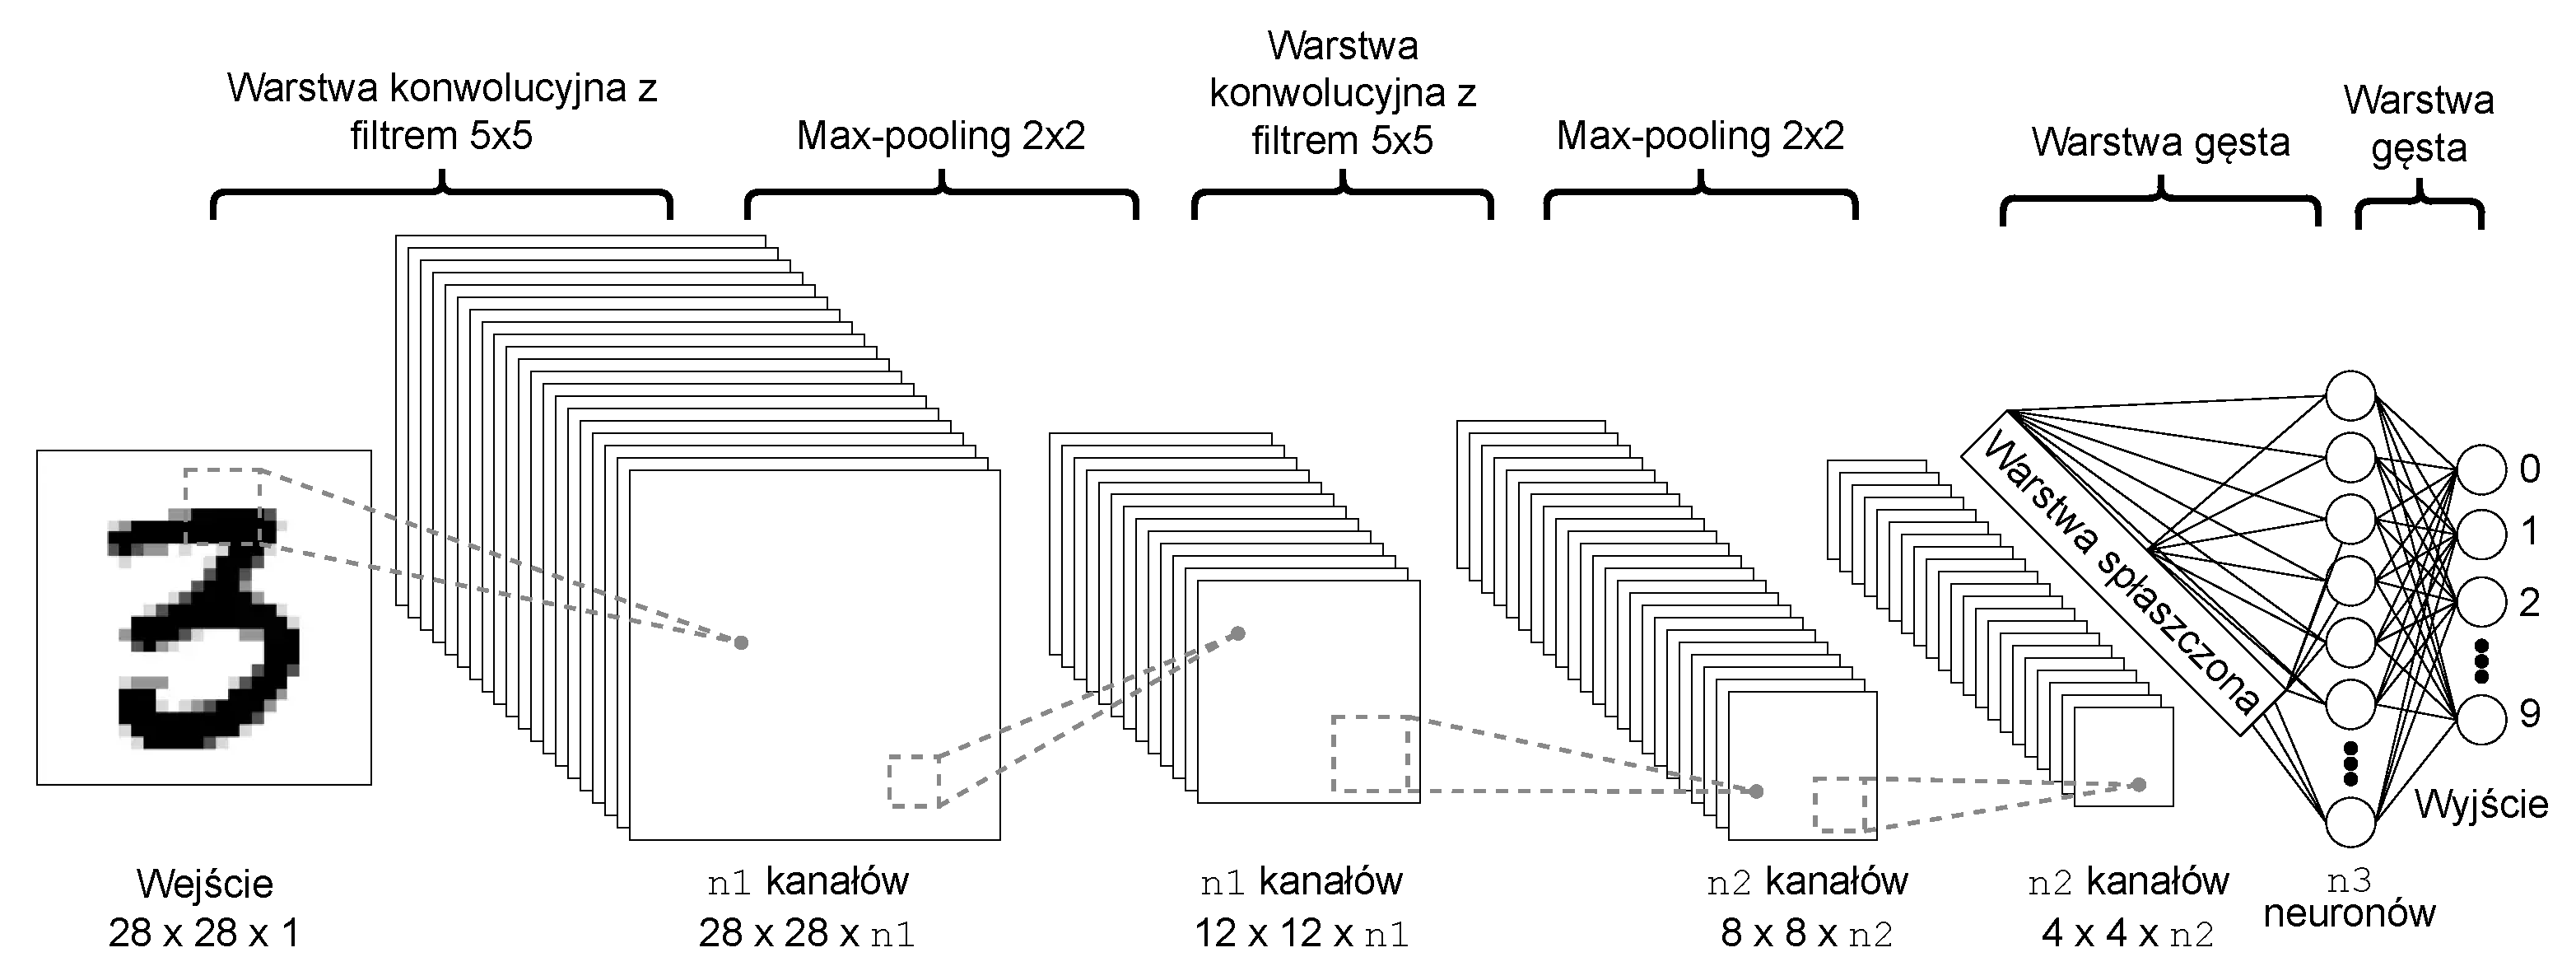
\includegraphics[width=\textwidth]{convolutional-neural-network-architecture}
  \caption[Przykładowa architektura konwolucyjnej sieci neuronowej]{Przykładowa architektura konwolucyjnej sieci neuronowej zaadoptowana z artykułu Sumita Saha na portalu \url{saturncloud.io} \cite{saha2018comprehensive}.}
  \label{fig:convolutional-neural-network-architecture}
\end{figure}

Na \hyperref[fig:convolutional-neural-network-architecture]{rysunku \ref*{fig:convolutional-neural-network-architecture}} przedstawiona jest przykładowa architektura konwolucyjnej sieci neuronowej zaadoptowana z artykułu na portalu \url{saturncloud.io} \cite{saha2018comprehensive}.
Sieć prezentuje system klasyfikacji obrazów ręcznie pisanych cyfr arabskich ze zbioru danych MNIST \cite{mnist}.

W niej dane wejściowe obrazu o wymiarach $28 \times 28 \times 1$ (czyli traktując macierz o wymiarach $28 \times 28$ jako tensor) przekazywane są najpierw do warstwy konwolucyjnej z $n1$ filtrami o rozmiarze $5 \times 5$.
Każdy filtr generuje swoją wynikową macierz o wymiarach $24 \times 24 \times 1$, a przez fakt, że użyto $n1$ filtrów, otrzymujemy tensor o wymiarach $24 \times 24 \times n1$.

Następna warstwa sieci to warstwa poolingowa, a dokładniej typu \emph{max-pooling}, która zmniejsza wymiary danych wejściowych.
Posiada ona \emph{okno poolingu} o wymiarach $2 \times 2$, które przesuwane jest po danych wejściowych z krokiem $2$ (tak, aby okna na siebie nie nachodziły).
Z każdego okna wybierana jest największa wartość, która jest następnie zapisywana w macierzy wyjściowej.
W ten sposób z danych wejściowych o wymiarach $24 \times 24 \times n1$ otrzymujemy macierz o wymiarach $12 \times 12 \times n1$.

Kolejna warstwa jest ponownie warstwą konwolucyjną o $n2$ filtrach o rozmiarze $5 \times 5$.
Każdy z $n1$ kanałów danych wejściowych (trzeci wymiar tensora) jest przetwarzany osobno przez każdy z filtrów i dla każdego generowany jest wyjściowy tensor o wymiarach $8 \times 8 \times n2$.
Następnie wszystkie $n1$ tensory są sumowane, tworząc pojedynczy tensor o wymiarach $8 \times 8 \times n2$ jako wyjście tej warstwy konwolucyjnej.

Kolejna warstwa to znów warstwa \emph{max-pooling} o wymiarach okna $2 \times 2$, która zmniejsza wymiary danych wejściowych z $8 \times 8 \times n2$ do $4 \times 4 \times n2$.

Później następuje spłaszczenie danych wejściowych do wektora o długości $4 \times 4 \times n2 = 16n2$ i przekazanie go do warstwy gęstej o $n3$ neuronach.
Połączenie między warstwą spłaszczoną a gęstą również jest w pełni połączone -- każdy z neuronów warstwy gęstej jest połączony z każdym z neuronów warstwy spłaszczonej.

Ostatnia warstwa gęsta ma $10$ neuronów, co odpowiada liczbie klas, na które ma być dokonywana klasyfikacja i jest jednocześnie warstwą wyjściową sieci.

\subsubsection{Przykłady zastosowań w analizie obrazów i diagnostyce medycznej}

Ne względu na swoją uniwersalność i skuteczność, głębokie uczenie maszynowe znalazło zastosowanie w wielu dziedzinach, w tym w analizie obrazów i diagnostyce medycznej.
Część algorytmów regresyjnych wykorzystywana jest do detekcji anomalii w sekwencjach danych różnego typu jak rytmu bicia serca, w tym także rekurencyjne sieci neuronowe i LSTM \cite{fernando2021deep}.
Jednak głębokie konwolucyjne sieci neuronowe są najczęściej wykorzystywane do analizy obrazów i diagnostyki medycznej lub detekcji nieprawidłowości bazującej na danych obrazowych.
Takie zastosowania również są często wykorzystywane i aktywnie rozwijane, a już na te chwilę osiągają bardzo dobre wyniki i pomagają w diagnozowaniu wielu chorób \cite{liu2017survey}.

Zakres zastosowań w medycynie, do których wykorzystywane są głębokie konwolucyjne sieci neuronowe jest bardzo szeroki.
Jest to przede wszystkim diagnostyka bazująca na obrazach rezonansu magnetyczne, tomografii komputerowej, czy też obrazach rentgenowskich.

Jednym z takich konkretnych zastosowań jest wykrywanie raka piersi na podstawie obrazów mammograficznych.
Badacze wykorzystali piramidową reprezentację Gaussa nazywaną też piramidową konwolucyjną siecią neuronową (ang. \emph{Pyramid-CNN}), wariant sieci CNN zbudowanej z coraz to mniejszych warstw konwolucyjnych przypominających strukturalnie piramidę \cite{bakkouri2019multi}.
Najszerszy poziom to warstwa wejściowa, a każda kolejna warstwa jest coraz węższa, aż do kategoryzujące warstwy wyjściowej.
Osiągnięte wyniki były bardzo obiecujące, gdzie system osiągnął średnią dokładność 96,84\%, czułość 92,12\%, swoistość 98,02\%, precyzję 92,15\%.

Innym przykładem zastosowań również z obszaru diagnostyki onkologicznej jest wykorzystanie głębokich konwolucyjnych sieci neuronowych do detekcji raka trzustki na podstawie obrazów tomografii komputerowej \cite{sekaran2020deep}.
Przestawione tam również było porównanie różnych metod uczenia maszynowego do tego samego zadania i na tych samych danych, gdzie najlepiej ze wszystkich uwzględnionych algorytmów wypadło głębokie konwolucyjne uczenie maszynowe.

Kolejnym przykładem jest wykorzystanie głębokich konwolucyjnych sieci neuronowych w zbudowaniu endoskopowej bazy wiedzy, która może być używana w podejściu opartym na zapytaniach \cite{petscharnig2018binary}.
Godne zauważenia tutaj jest, że system był uczony na materiałach wideo i na takich również miał za zadanie operować.
Wykorzystując bazę nagrań endoskopowych gromadzonych w trakcie operacji przez chirurgów badaczom udało się zbudować system, który potrafił poprawnie odpowiadać na dobrze skonstruowane zapytania.
Pokazali również, że cechy zbudowanego przez nich modelu CNN są kompaktowymi, ale wydajnymi deskryptorami obrazu do wyszukiwania w domenie obrazowania endoskopowego.
Są one w stanie utrzymać najnowocześniejszą wydajność, zapewniając jednocześnie korzyści w postaci niskiego zapotrzebowania na miejsce do przechowywania, a tym samym zapewniają najlepszy kompromis.

Pomimo wielu pozytywów warto jednak również zauważyć, że medycyna jest dziedziną z niesamowicie małym marginesem błędu oraz gdzie nawet skuteczne rozwiązania nie będące w pełni przetestowane pod względem ich bezpieczeństwa i skuteczności są odrzucane.
Między innymi to jest powodem, dla którego wdrożenie rozwiązań głębokiego uczenia maszynowego jest tak czasochłonne i często budzi również kontrowersje.
Metody uczenia maszynowego nazywane są ``czarnymi skrzynkami'', ponieważ poza wyjaśnieniem doboru architektury, procesu uczenia sieci i algorytmu za nim stającym nie jest możliwe wyjaśnienie, dlaczego sieć dokonuje takich, a nie innych predykcji, co jest problematyczne w obszarze opierającym się na pełnej pewności bezpieczeństwa używanych rozwiązań \cite{pouyanfar2018survey}.

\subsection{Uczenie transferowe i wstępnie wytrenowane modele sieci neuronowych}
\label{sec:transfer-learning}

Uczenie transferowe to technika uczenia maszynowego, która polega na wykorzystaniu wiedzy zdobytej z jednego zadania w celu poprawienia wyników innego, pokrewnego zadania.
To potężne podejście stosowane w sytuacjach, gdzie dane dla celowego zadania są ograniczone, a dostępne są obfite dane dla zadania źródłowego, które jest powiązane.

Technika ta ma wiele zalet, przede wszystkim prędkość trenowania -- ``dotrenowanie'' modelu wykorzystujące inny, wstępnie wytrenowany model jest znacznie szybsze niż trening podobnego modelu od zera.
Wykorzystuje on bowiem wiedzę zgromadzoną w modelu źródłowym, który został już wcześniej wytrenowany na ogromnych zbiorach danych.
Dodatkowo efektywne wykorzystane są dane, trenowanie modelu używając uczenia transferowego wymaga znacznie mniej danych wejściowych niż trenowanie modelu od zera \cite{weiss2016survey}.

Zalety te opierają się na jednej zasadniczej cesze wstępnie wytrenowanego modelu -- jest on uczony w taki sposób, aby wytworzyć reprezentacje bardzo uniwersalne, które są w stanie uchwycić wiele różnych cech w danych wejściowych określonego typu.
Innymi słowy posiada już zgeneralizowaną wiedzę na temat ogólnej kategorii danych, dla których jest przeznaczony.
Przykładowo model dedykowany jako baza w kategoryzacji obrazów będzie miał umiał w bardzo ogólny sposób analizować obrazy prowadząc do takiego reprezentacji, aby posiadała jak najwięcej informacji o cechach obrazu w sposób uniwersalny.
Następnie doszkalany model bazowany na tym już wstępnie wytrenowanym wyłącznie wykorzystuje te bogate reprezentacje cech oferowane przez rdzenny model do kategoryzacji obrazów wybranego rodzaju, na przykład odróżnianie obrazów psów od kotów.

Modele wstępnie wytrenowane są zazwyczaj ogromnie i mają bardzo złożoną architekturę.
Zadanie generalizowania obszaru problemowego dla problemów, które nie są jeszcze znane jest bowiem bardzo trudne, co odzwierciedla wielkość takich sieci.

Dla przykładu jedną z popularnych wykorzystywanych wstępnie wytrenowanych sieci neuronowych stosowanych w zadaniach analizy obrazu jest \emph{ResNet} (\emph{Residual Neural Network}).
Jego architektura zaczyna się od standardowego bloku konwolucyjnego i normalizującego, jednak następnie posiada kluczowe dla swojego działania specjalne \emph{bloki resztkowe} (inaczej \emph{rezydualne}, z ang. \emph{residual blocks}) \cite{li2016demystifying}.
Blok resztkowy składa się z co najmniej dwóch konwolucyjnych warstw, które przetwarzają dane wejściowe, a następnie ich wynik jest dodawany do oryginalnych danych wejściowych.
To dodanie pozwala na przekazywanie reszty (różnicy) między oryginalnymi danymi a przetworzonymi danymi przez blok resztkowy.
Dalej składa się ponownie z klasycznie używanych bloków takich jak warstwy poolingowe czy gęste, aż do warstwy wyjściowej.

Dzięki swojej blokowej budowie w zależności od potrzeb można wykorzystać różne warianty sieci ResNet, które różnią się głębokością sieci.
Dostępne są modele \emph{ResNet-18}, \emph{ResNet-34}, \emph{ResNet-50}, \emph{ResNet-101}, \emph{ResNet-152} oraz \emph{ResNet-200}, gdzie liczba w nazwie oznacza liczbę warstw w sieci.
